\section*{1. Coordinate system}

a) Define \textbf{zenith}, \textbf{nadir}, the \textbf{celestial north} and \textbf{south poles}, and the
\textbf{meridian line}. Draw the meridian plane of an observer, including the position of the observer 
(*), the zenith (Z), the meridian line, and the north (N) and south (S) poles.\\
\\
\begin{itemize}
    \item \textbf{zenith}: Point which is directly over the observer on a celestial sphere
    \item \textbf{nadir}: Point which is directly under the observer on a celestial sphere
    \item \textbf{celestial north pole}: Northern point of the Earth's rotation axis
    \item \textbf{celestial south pole}: Southern point of the Earth's rotation axis
    \item \textbf{meridian line}: Great circle that passes through the celestial poles
\end{itemize}

\noindent\makebox[\textwidth]{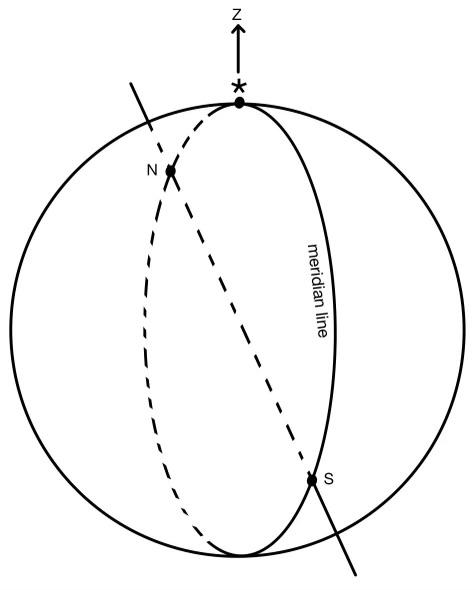
\includegraphics[scale=0.35]{meridian_plane.jpeg}}
\noindent
b) An observer located in the Earth's Northern Hemisphere observers the top and bottom culminations of
circumpolar star. Measuring $h_i = 20 \degree \: 22' \: 32.4''$ ; $A_i = 180 \degree$ for the hight and
Azimuth of the bottom culmination and $h_s = 50 \degree \: 23' \: 08.2''$ ; $A_s = 180 \degree$ for the
upper culmination. What is the observer's latitude $\phi$?\\
\\
First of all we convert the measured hights:
\begin{equation*}
    \begin{split}
        h_i &= 20 \degree \: 22' \: 32.4''\\
            &= 20 \degree + \frac{22 \degree}{60} + \frac{32.4 \degree}{3600}\\
            &\approx 20 \degree + 0.36666667 \degree + 0.009 \degree\\
            &= 20.37566667 \degree\\
        h_s &= 50 \degree \: 23' \: 08.2''\\
            &= 50 \degree + \frac{23 \degree}{60} + \frac{08.2 \degree}{3600}\\
            &\approx 50 \degree + 0.38333333 \degree + 0.00227778\degree\\
            &= 50.3856111 \degree\\
    \end{split}
\end{equation*}

\noindent
c) Determine the maximum height in the sky that the globular cluster $\omega$Cen (declination 
$\delta = -47 \degree \: 29'$) reaches when observed from the Inter-American Observatory of Cerro Tololo,
Chile (latitude $\phi = -30 \degree \: 10' \: 20.9''$)\\
\\
